\documentclass[../main.tex]{subfiles}
\graphicspath{{\subfix{../img/}}}
\begin{document}

\newpage
\section{Einleitung}

In den kommenden Jahren wird autonomes Fahren zunehmend an Bedeutung gewinnen. Diese Arbeit beschäftigt sich mit den ersten Entwicklungsstufen dieser Technologie. Ziel des Projekts ist es, ein autonomes Fahrzeug zu entwickeln, das Hindernisse und Veränderungen in einem vorgegebenen Wegenetz flexibel meistern kann. Das Team besteht aus Studierenden der Elektrotechnik, Informatik und Maschinenbau. Dadurch wird die interdisziplinäre Zusammenarbeit gefördert. Dabei setzt das Team theoretisches Wissen in praktische Anwendungen um und entwickelt innovative Lösungen. Der Fokus liegt dabei nicht nur auf der technischen Umsetzung, sondern auch auf Nachhaltigkeit und einer umfassenden Dokumentation des Entwicklungsprozesses.

Das Fahrzeug soll sich in einem Wegenetz mit acht fixen Wegpunkten orientieren, Hindernisse erkennen, gesperrte Punkte umgehen und auf entfernte Streckenabschnitte reagieren können. Das Ziel dabei ist, den Zielpunkt schnell und effizient zu erreichen, ohne die Herausforderungen der Umgebung aus den Augen zu verlieren.
\begin{figure}[H]
    \centering
    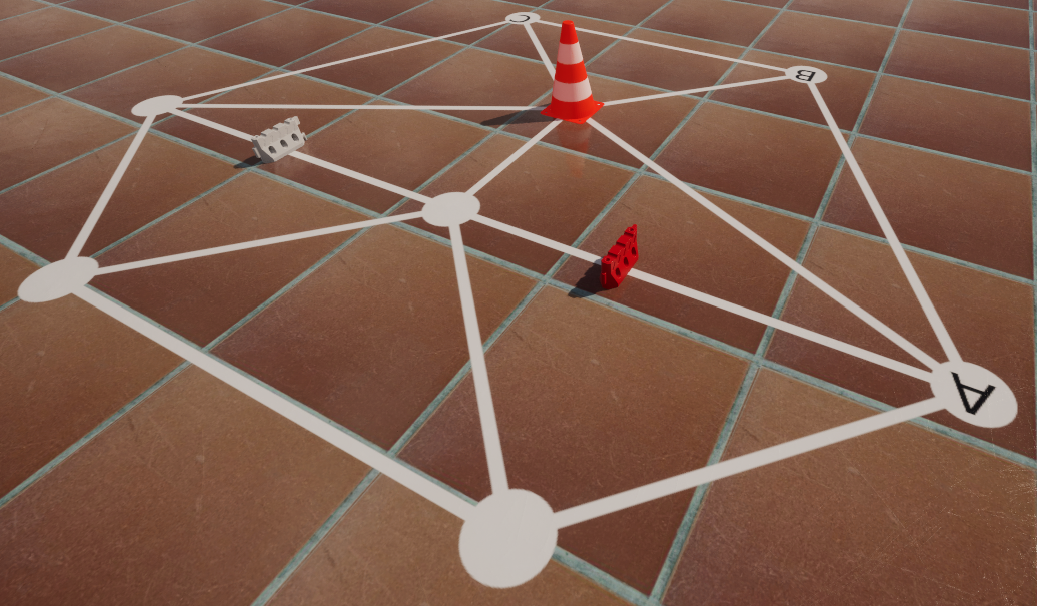
\includegraphics[width=0.75\linewidth]{img/unrealengine/unreal.png}
    \caption{Digital Twin des Problem-Szenarios. Realisiert mit Unreal Engine\protect\footnotemark.}
    \label{intro_digital_twin}
\end{figure}
\footnotetext{\href{https://www.unrealengine.com/}{https://www.unrealengine.com/}}
Das Projekt besteht aus zwei Phasen:

\textbf{Herbstsemester (\acrshort{pren1}):} Entwicklung eines Gesamtkonzepts mit Simulator zur Planung von Fahrwegen und Reaktionen auf Hindernisse. Fokus liegt auf Planung und Dokumentation.
\textbf{Frühlingssemester (\acrshort{pren2}):} Bau eines Prototyps, basierend auf dem Konzept. Der Prototyp wird im Wettbewerb auf Zuverlässigkeit, Effizienz und Regelkonformität getestet.
Nachhaltigkeit ist ein zentraler Aspekt, einschliesslich Materialwahl und Recycling. Der Projektverlauf dokumentiert nachhaltige Aspekte und dient als Beispiel für künftige Projekte.

Die originale Aufgabenstellung befindet sich im Anhang \ref{aufgabenstellung}.
\newpage

Der erste Schritt der Vorgehensweise ist die Informationsbeschaffung, für die eine Technologierecherche durchgeführt wurde (siehe Anhang \ref{technologierecherche}). Auf Basis der gewonnenen Erkenntnisse wurde anschliessend ein morphologischer Kasten entwickelt, der in verschiedene Teilfunktionen unterteilt ist. Jede Teilfunktion wird durch verschiedene Lösungsoptionen abgedeckt (siehe Anhang \ref{morphologischer kasten}).

Aus dem morphologischen Kasten ergaben sich zwei Lösungskonzepte, die im Anhang \ref{a3:loesungsvariante_Simpel} detailliert beschrieben sind. Zur Auswahl der geeignetsten Lösung wurden die einzelnen Komponenten getestet; die Testergebnisse sind im Anhang \ref{a4:prototyping} dokumentiert. Die letztendlich gewählte Lösung wird im Hauptteil dieser Arbeit ausführlich beschrieben. Weitere Details zur Entscheidungsfindung und zu den Lösungsoptionen finden sich in den genannten Anhängen.


\subsection{Skizze Aufgabenstellung}
Die Skizze soll die Aufgabenstellung visuell darstellen und dadurch eine  Übersicht über die einzelnen Anforderungen und Funktionen des Fahrzeuges schaffen.
    \begin{figure}[H]
        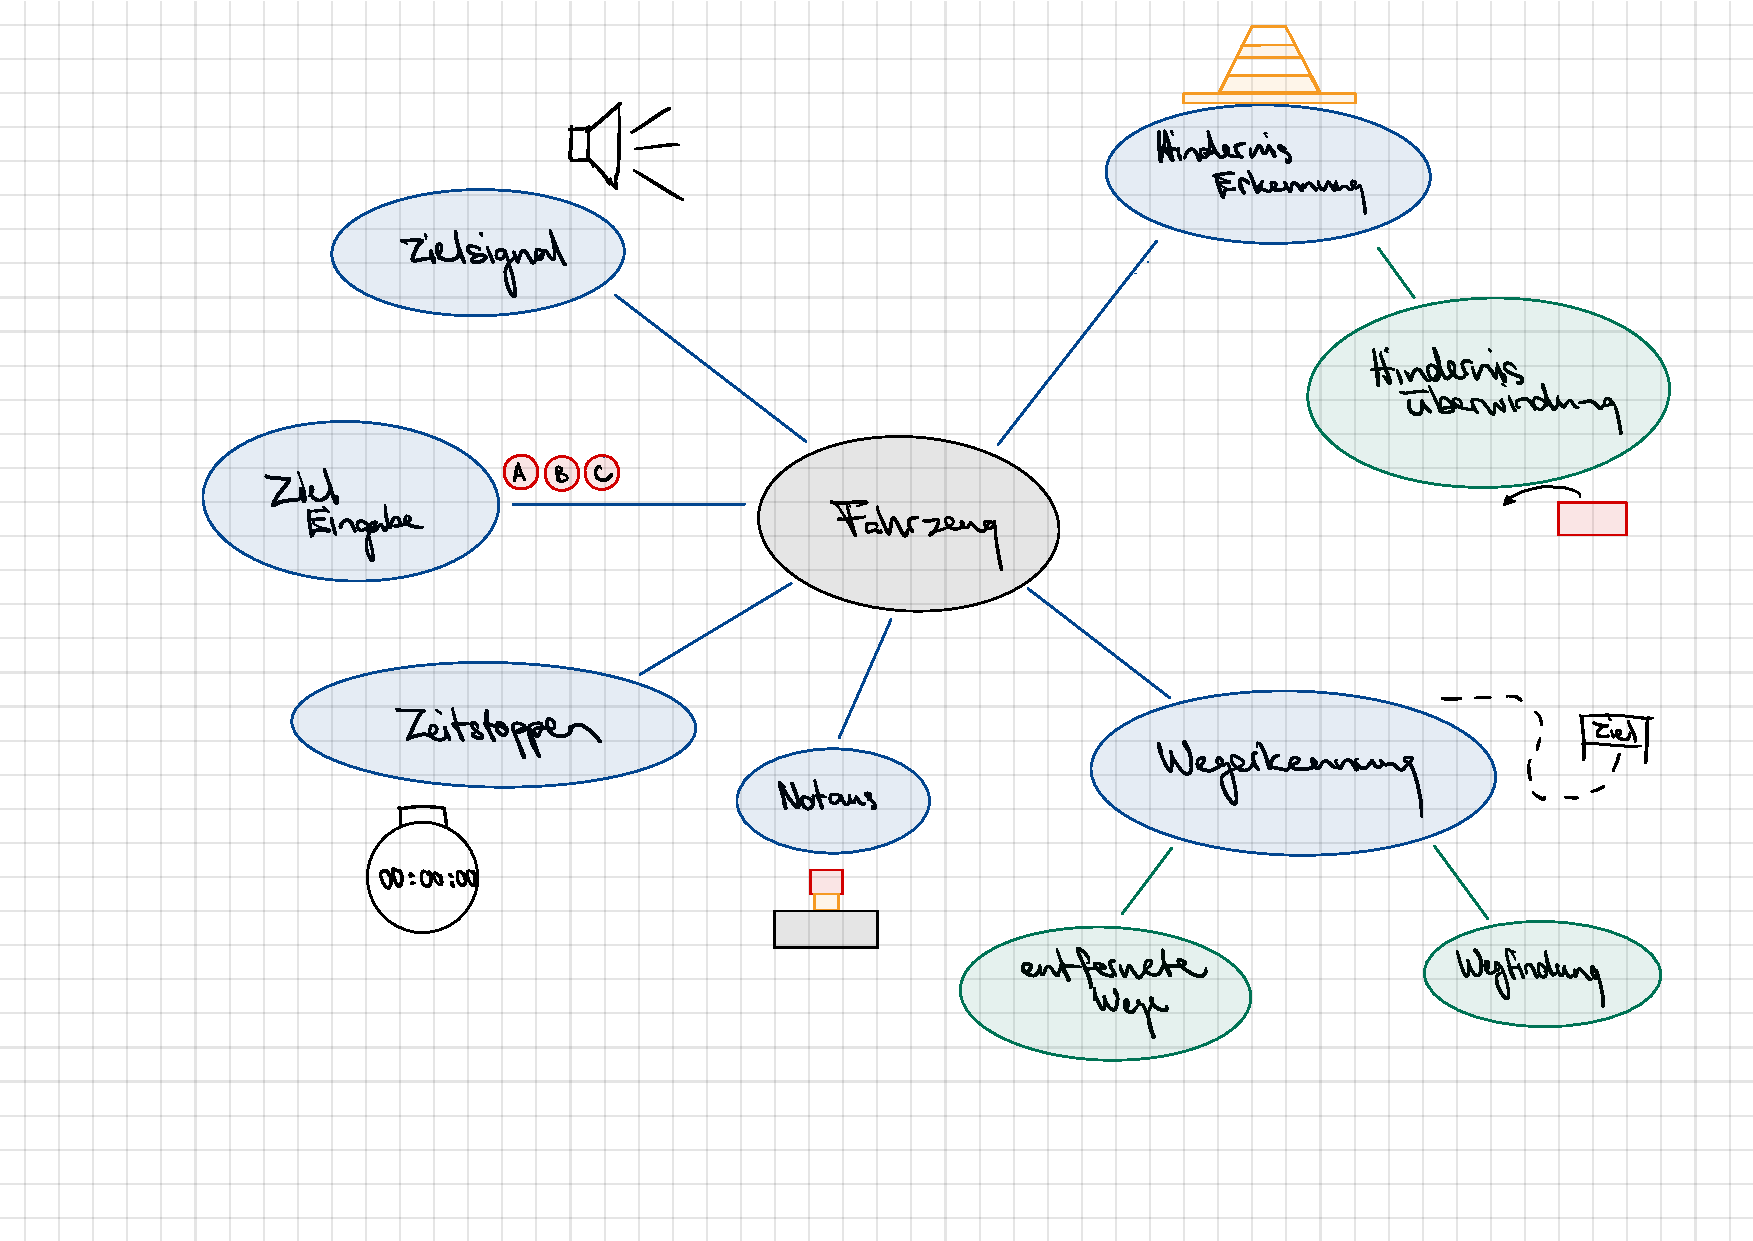
\includegraphics[width=\textwidth]{assets/Skizze_Aufgabenstellung.pdf}
        \caption{Skizze der Aufgabestellung}
        \label{img:Skizze_Aufgabenstellung}
    \end{figure} 
 
\end{document}